%--------------------------------
\section{Discussion}
\label{cap6_discussion}

The experiments carried out in the KITTI data set allowed the conclusion that adding side-outputs in the network helps both the performance and the convergence during the training phase.
%It was also observed that the increase in network performance was directly related to the increase in the number of side-outputs.
It was also possible to directly relate the increase in network performance with the increase in the number of side outputs.

The results obtained in Section \ref{cap6_experm_1_qtd_saidas} indicated equivalence between side-output merging operations.
However, as verified later in Section \ref{ssec:basic_pred_eval}, the MAX operation performed considerably less than the ADD and AVG.
The first results, which indicated similar performances, can be attributed to the relative simplicity of highway segmentation when compared to the edge detection, a much more complex and accurate task.

%As verified in Section \ref{cap6_contribuicoes_saidas_intermediarias} and later in Section \ref{ssec:bsds_sideout}, network learning is influenced by the method used to combine the outputs.
As verified in Section \ref{ssec:bsds_sideout}, network learning is influenced by the method used to combine the outputs.
After the individual assessment of the contribution of each of the stages, in Section \ref{ssec:bsds_subexp3}, it was possible to reduce the network, eliminating layers with small contributions to the result.

To train the network on the BSDS500 data set, it was necessary to change the loss function to help with the imbalance between borders and non-borders pixels.
% Due to imbalance between classes, the \textit{Categorical Cross Entropy} function had difficulties in converging, becoming inadequate.
% To help with the imbalance, \textit{Focal Loss} function was chosen.
After some tests, it was observed that \textit{Focal Loss} could learn edges but produced mostly soft borders\footnote{~This condition was also reported in the work of \cite{WangDOOBNet:2018}, analyzed later.}.
From small experiments, it was possible to notice that the increase in the difference in tone between edge and background pixels allowed a faster network convergence.
In this way, edge pixels were binary classified, regardless of the number of times they appeared in multiple ground truths.

However, multiple ground truths when placed overlapping, caused noise and thick edges.
To solve this problem, a detailed study of the ground truth was carried out and a framework for experiments was created.
In the framework protocol, the first phases uses large differences between the pixels, with morphological thinning operation to reduce noise, while in the following phases the differences were more subtle, which made it possible to refine the results.

% In order to increase the convergence of the Focal Loss function, a small change was made to add an extra parameter, corresponding to the Pixel Error metric, also used in the KITTI data set experiments.
% The change, despite improving the network convergence, the new PEFL function, did not considerably improve the smooth identification of sets.

Due to the smooth identification of edges, the network, despite the good results in the ODS and OIS metrics, presented low results in the AP metric, when compared to other methods in the literature.
It can also be inferred from the PR curve of Figure \ref{fig:bsds_xlo_avg_curve} that the network does not distinguish the edges well, being necessary to consider low thresholds as edges. 
Low thresholds between borders and background have also been adopted in other studies, such as the DOOBNet network \cite{Cumulative:Song20181847}.

\begin{figure}%[h!]
  \centering
  \includegraphics[width=0.9\columnwidth]{../imagens/graficos/cap6_xlo-avg.png}
  \caption{\color{red}Precision Recall curve for XLO-AVG network (ALL ground truth).}
  \label{fig:bsds_xlo_avg_curve}
\end{figure}

\begin{comment}
\begin{table}%[h!]
  \centering
  \caption{Performance comparison between our method and other methods in literature.}
  %\scriptsize
  %\setlength{\tabcolsep}{1em}
  \renewcommand{\arraystretch}{1.5}
  \begin{tabular}{{l}{c}{c}{c}}
    \hline
    Method & ODS & OIS & AP
    \\
    \hline
    DeepContour \cite{DeepContour:2015:7299024} & .756 & .776 & -
    \\
    HED \cite{HED:2015} & .782 & .808 & -
    \\
    DCNN + sPb \cite{Kokkinos:2016} & .813 & .831 & -
    \\
    RDS \cite{LearningRelaxed:2016:7780401} & .792 & .810 & -
    \\
    EdgeNet \cite{SemanticSeg:2016:7780861} & .718 & .731 & -
    \\
    Edge CNN \cite{EdgeCNN:Wang201612} & .69 & .71 & -
    \\
    COB \cite{COB:2016} & .793 & - & -
    \\
    \cite{Wang:2017} & .803 & - & -
    \\
    \cite{ContourDetect:2017:8124495} & .75 & - & -
    \\
    \cite{DeepStructured:2017:Xu20173962} & .798 & - & -
    \\ 
    RCF \cite{RCF:2017:8100105} & .819 & .823 & -
    \\
    \cite{ProeminentEdge:2018:Cai2018} & .788 & - & -
    \\ 
    \cite{Cumulative:Song20181847} & .819 & - & -
    \\
    \cite{CrispBoundaries:2018:Deng2018570} & .815 & - & -
    \\ 
    \cite{ReExtraction:Wen201884} & .804 & - & -
    \\  
    \cite{LearningHybrid:Hu2018377} & .814 & - & -
    \\
    \cite{Yang:2019} & .810 & - & -
    \\
    BDCN \cite{He:2019} & .828 & .844 & -
    \\
    \hline
    XLO-ADD (ALL) & .776 & .790 & .702
    \\
    XLO-ADD (UPPER) & .774 & .790 & .685
    \\
    XLO-AVG (ALL) & .780 & .793 & .721
    \\
    XLO-AVG (UPPER) & .780 & .796 & .700
    \\
    \hline
  \end{tabular}
  \label{tab:bsds_subexp5_results}
\end{table}
\end{comment}

% \begin{figure}%[h!]
%   \centering
%   \subfloat[\label{sfig:bsds_xlo_avg_curve}]{\includegraphics[width=0.48\textwidth]{imagens/graficos/cap6_xlo-avg.jpg}}
%   \hfill
%   \subfloat[\label{sfig:literature_curves}]{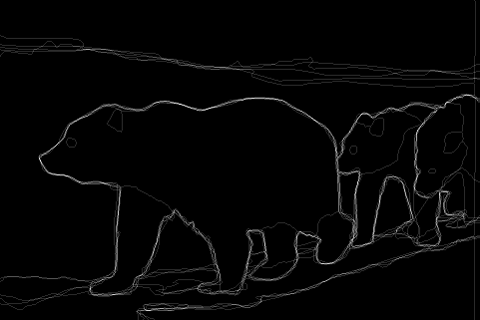
\includegraphics[width=0.48\textwidth]{imagens/ilustracoes/cap6_bsds_100075_all.png}}
%   \caption{(a) Precision Recall curve for XLO-AVG network (ALL ground truth) and (b) literature curves.}
%   \label{fig:bsds_xlo_avg_curve}
% \end{figure}

Based on the training protocol created, it was possible, in the last experiments, to indicate the superiority of the AVG when contrasted with ADD operation for merging the side-outputs of the network.
% The results obtained in both Sections \ref{ssec:bsds_subexp4} and \ref{ssec:bsds_subexp5} indicate that the AVG method produced better results and converged, in all tests carried out, with fewer training epochs.

%In Section \ref{ssec:bsds_subexp4}, experiments were developed to evaluate \textit{Hypothesis H3} and \textit{Research Question Q2}.
%From the results, it can be said that it is possible to generate good results without the need to train the neural network in order to produce similar results in each layer / stage.

Regarding the training epochs on the BSDS500 data set, all networks converged with less than 700 epochs (the best ODS result converged in 442 epochs).
Despite the low number of epochs, the number of images processed due to data augmentation was really high.
% Thus, to reduce the number of iterations, random subsets of images can be used each time, and the optimizer in the first phase of the protocol and the early stopping criterion can be changed.

Due to the good results produced by the ALO and XLO networks, post-processing methods were not performed on the results of the BSDS500 data set.
The usage of post-processing methods had little chance of improving the overall performance, being unjustified.
% In addition to satisfactory results, the use of post-processing methods had little chance of improving the final result, being unjustified.
% Post-processing methods also could decrease the network speed, which is a virtue of this work when compared to other methods in the literature.

%LIDOS
%\cite{DosSantos:2019} - Modelo de Cores (RGB, LAB, LUV)
% \cite{Wang:2019} - Mostra saídas laterais, manchas de baixa precisão, mas não tem BSDS. Contém saídas laterais
% \cite{Fu:2019} - Adição de pesos nas saídas laterais, para melhor desempenho (sem BSDS).
% \cite{LocalDepth:2017:8265527} - Verificação de aprendizado de redes neurais x humanos
% SHADOW EVALUATION >> Avalia pixels com valores entre 0.2 e 0.5. Esses valores geram um coeficiente que é utilizado na perda

%--------------------------------
